%TODO proof-of-concept
\textbf{Proof-of-Concept}.
We test the feasibility of {\shortname} and the results are shown from Fig.~\ref{fig:SPSC} to Fig.~\ref{fig:device}. In each figure, we show both the raw signal and the spectrogram for the microphone data and the motion sensor data. All data are collected by Google Nexus 6P. The audio data is sampled at  8,000 Hz (telephone quality) while the motion data is sampled at 400 Hz as it is the highest sampling rate on Nexus 6P.


Fig.~\ref{fig:SPSC}, Fig.~\ref{fig:DPSC}  and  Fig.~\ref{fig:SPDC}, show the example data when the same user speaks the same command ``Ok google'', different users speak the same command ``Ok Google'', and the same user speaks different commands ``Ok google'' and ``Hi Siri'', respectively. The data are collected as in Fig~\ref{fig:usec}.  In each figure, the top subfigure (a) is the raw microphone data; the subfigure (b) contains the 3-axis accelerometers data and 3-axis gyroscopes data; the subfigure (c) shows the frequency-domain information of raw audio data while the subfigure (d) show that of raw motion data. In subfigure (d),  we  only choose acc-z data to draw since it is the most representative one. The vertical red lines demonstrate the start and end points of the sounding period.

\newpage
%TODO figures about challenges
\begin{figure}[H]
	\centering
	\begin{minipage}[t]{.8\linewidth}
		\centering
		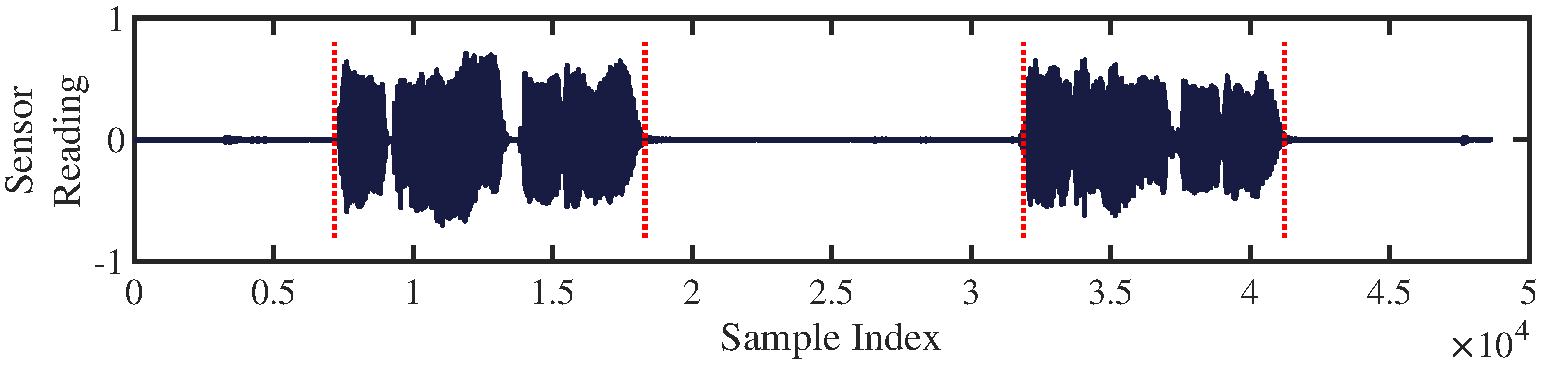
\includegraphics[width=\linewidth]{SPSC0}
		\vspace{-.2in}
		\subcaption{Raw Audio Data.}
		\vspace{.2in}
		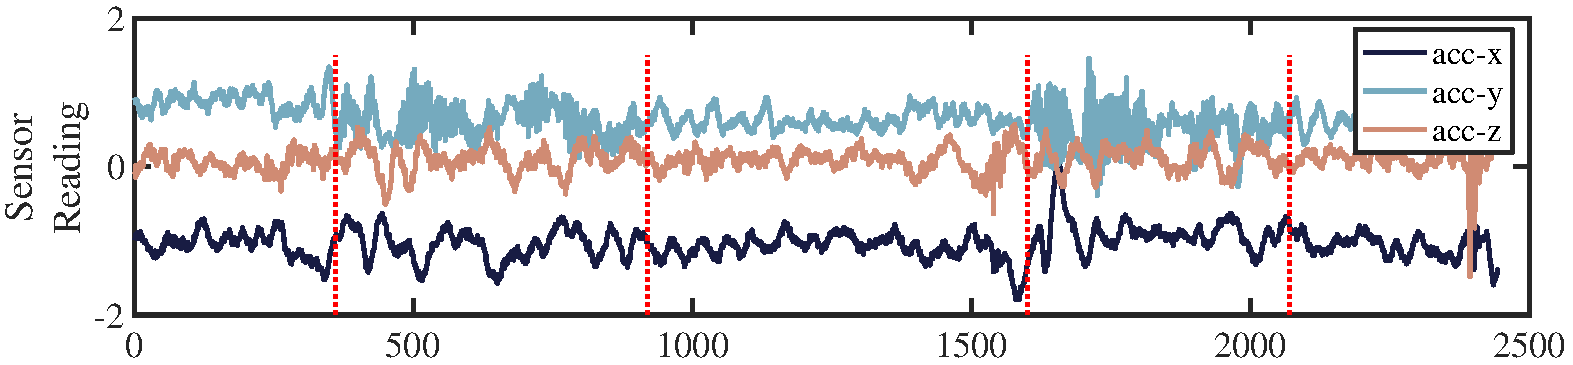
\includegraphics[width=\linewidth]{SPSC1}
		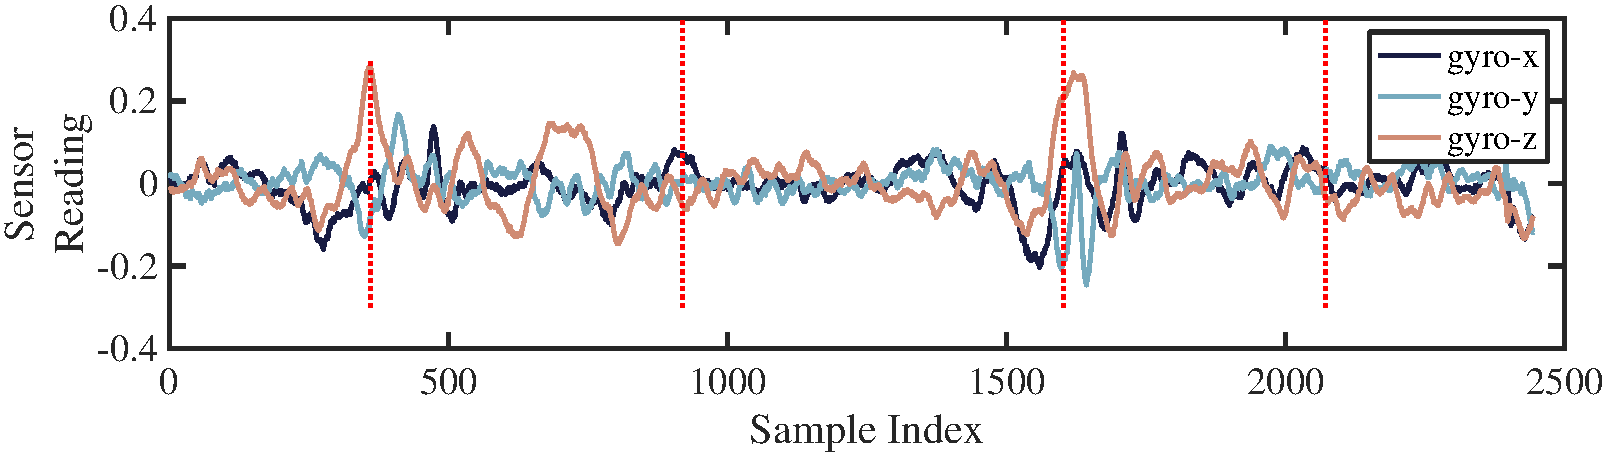
\includegraphics[width=\linewidth]{SPSC2}
		\vspace{-.2in}
		\subcaption{Raw Motion Data.}
		\vspace{.2in}
	\end{minipage}
	\begin{minipage}[t]{.45\linewidth}
		\centering
		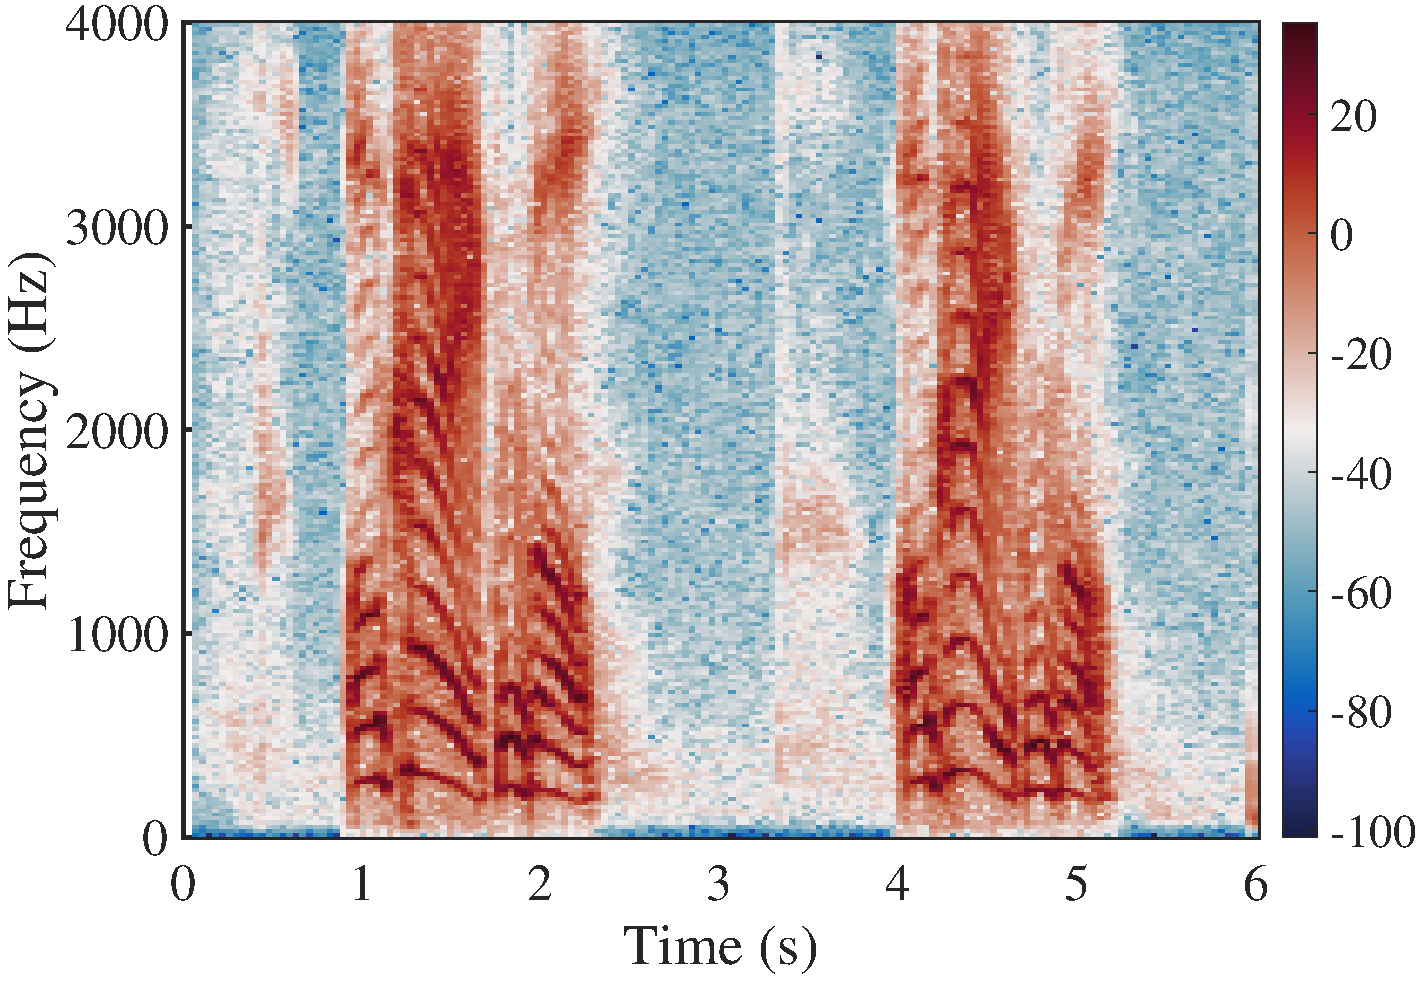
\includegraphics[width=\linewidth]{SPSC3}
		\vspace{-.2in}
		\subcaption{Spectrogram of Raw Audio Signals.}
	\end{minipage}
	\begin{minipage}[t]{.45\linewidth}
		\centering
		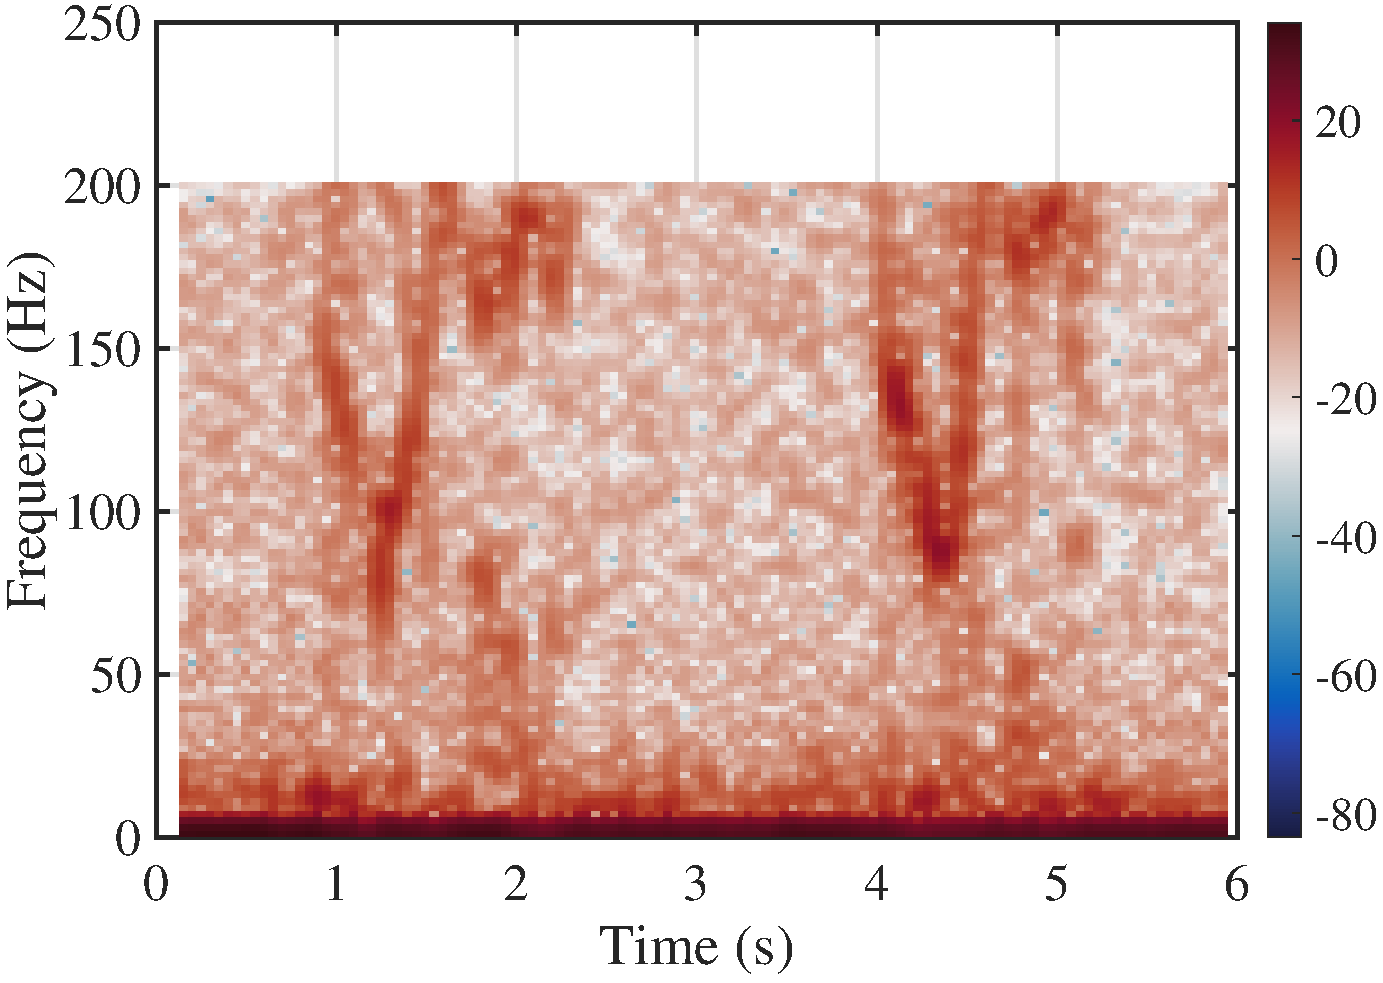
\includegraphics[width=\linewidth]{SPSC4}
		\vspace{-.2in}
		\subcaption{Spectrogram of Raw Motion Signals.}
	\end{minipage}
	\caption{One user speaks ``Ok Google'' twice.}
	\label{fig:SPSC}
\end{figure}
%
\newpage
\begin{figure}[H]
	\centering
	\begin{minipage}[t]{.8\linewidth}
		\centering
		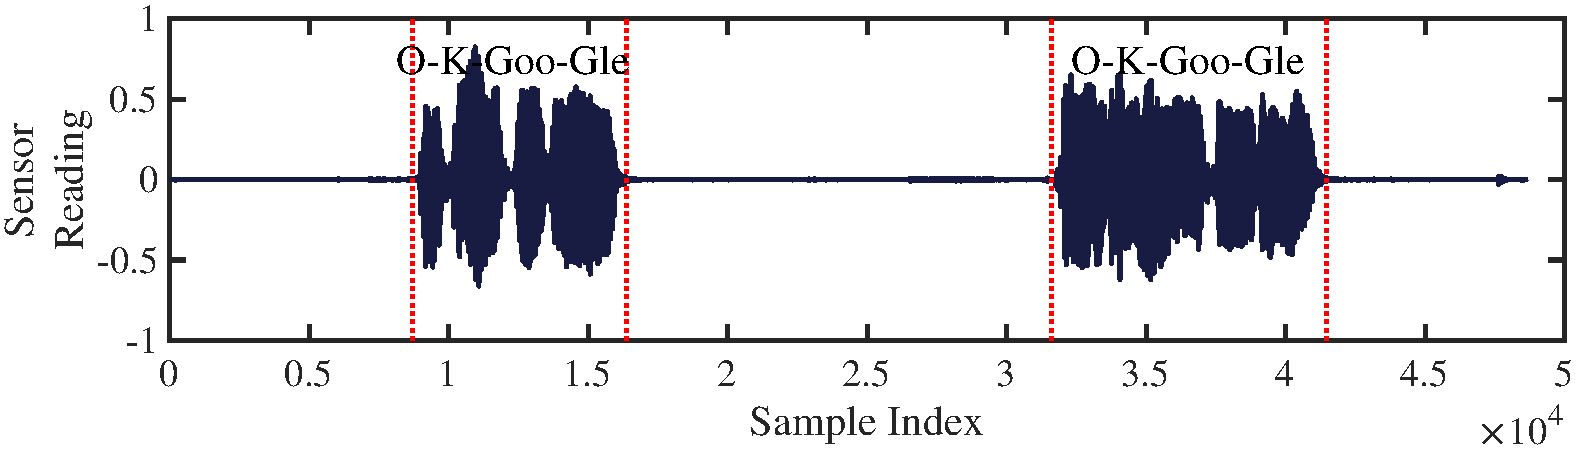
\includegraphics[width=\linewidth]{DPSC0}
		\vspace{-.2in}
		\subcaption{Raw Audio Data.}
		\vspace{.2in}
		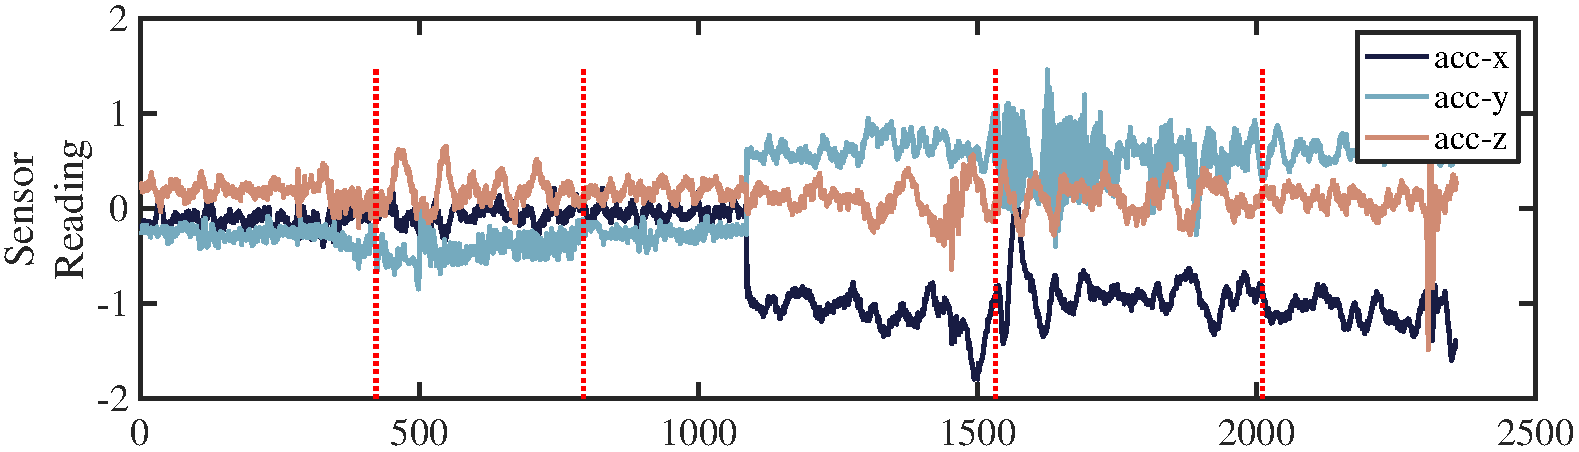
\includegraphics[width=\linewidth]{DPSC1}
		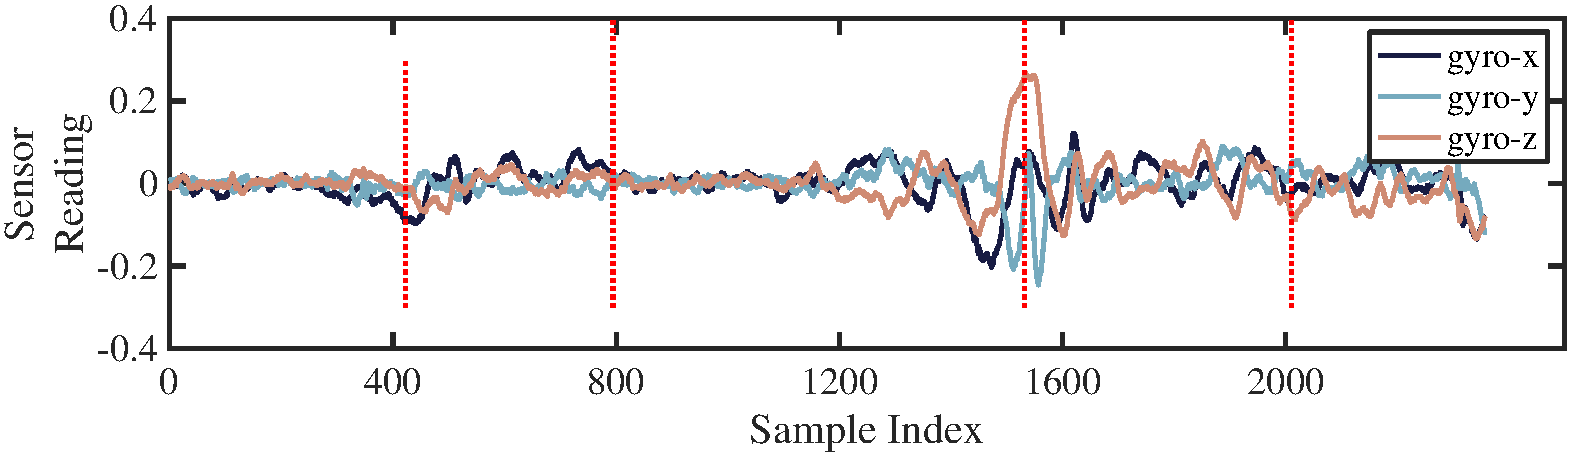
\includegraphics[width=\linewidth]{DPSC2}
		\vspace{-.2in}
		\subcaption{Raw Motion Data.}
		\vspace{.2in}
	\end{minipage}
	\begin{minipage}[t]{.45\linewidth}
		\centering
		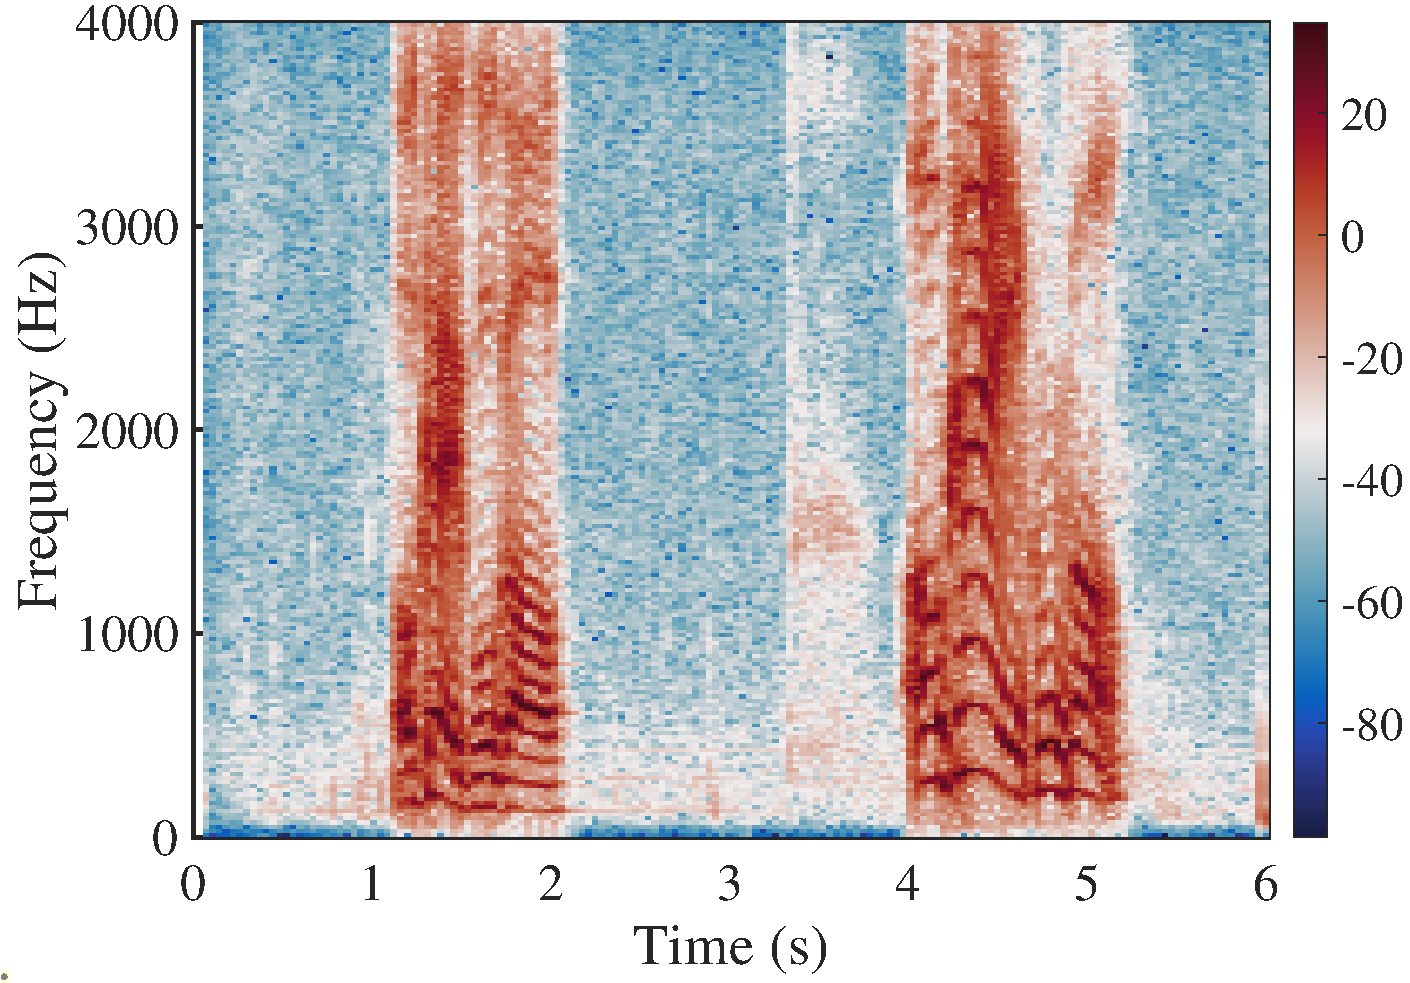
\includegraphics[width=\linewidth]{DPSC3}
		\vspace{-.2in}
		\subcaption{Spectrogram of Raw Audio Signals.}\label{fig:DPSCc}
	\end{minipage}
	\begin{minipage}[t]{.45\linewidth}
		\centering
		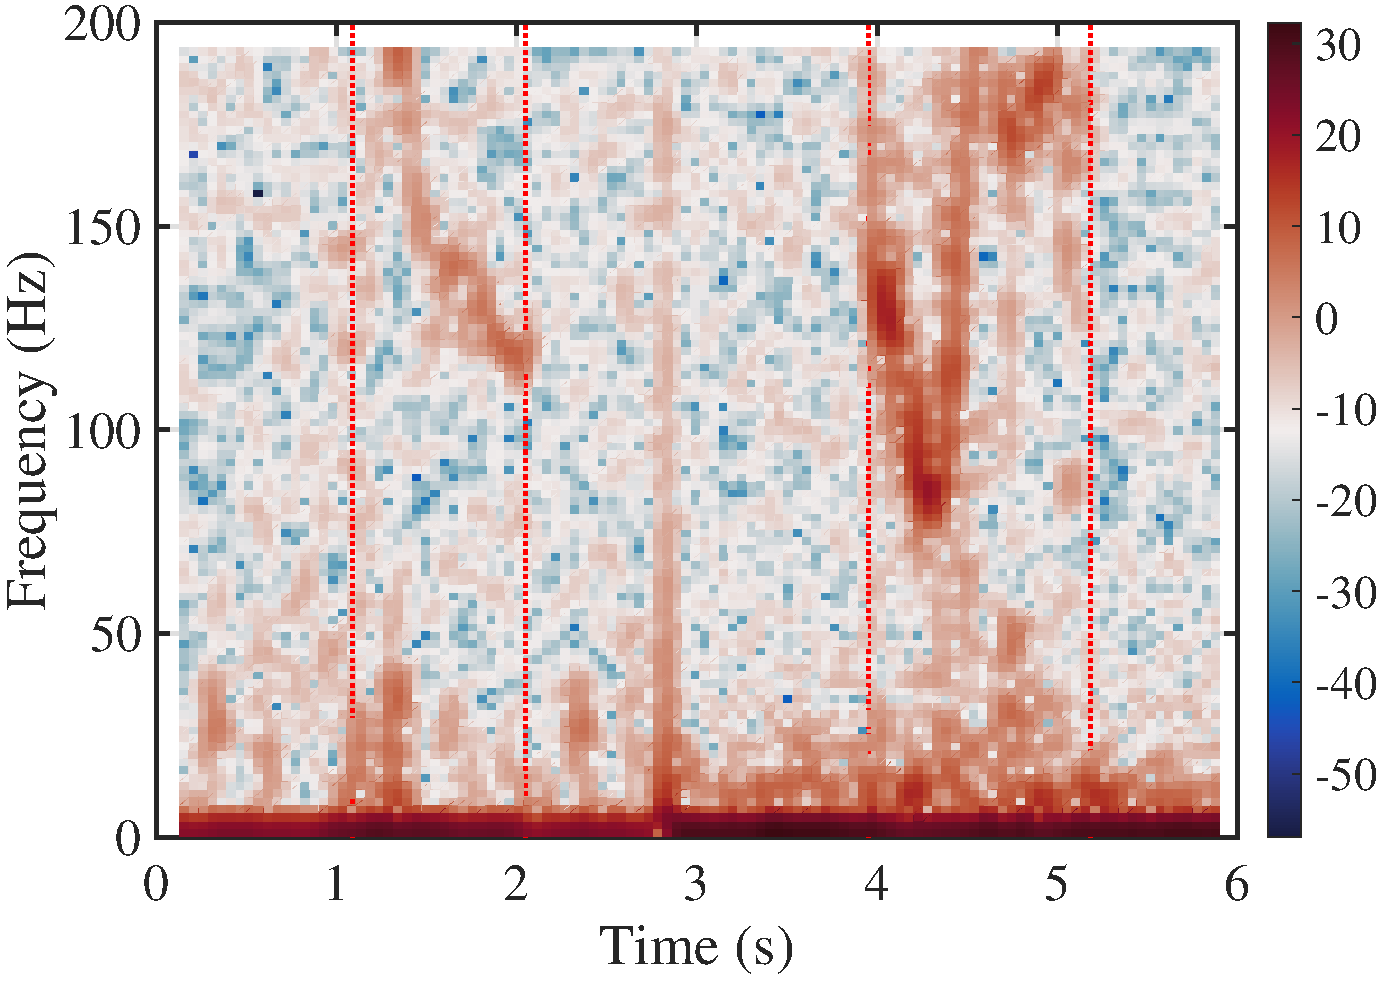
\includegraphics[width=\linewidth]{DPSC4}
		\vspace{-.2in}
		\subcaption{Spectrogram of Raw Motion Signals.}\label{fig:DPSCd}
	\end{minipage}
	\caption{Different users both speak ``Ok Google''.}
	\label{fig:DPSC}
\end{figure}
%TODO more descriptions about the figure.
\newpage
\begin{figure}[H]
	\centering
	\begin{minipage}[t]{.8\linewidth}
		\centering
		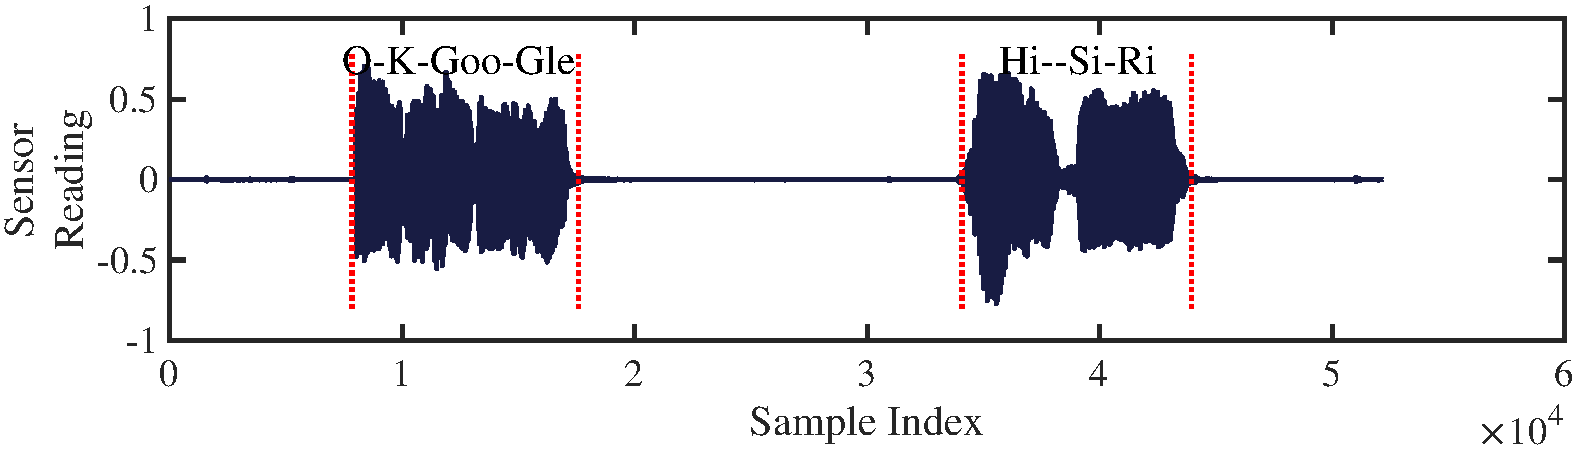
\includegraphics[width=\linewidth]{SPDC0}
		\vspace{-.2in}
		\subcaption{Raw Audio Data.}
		\vspace{.2in}
		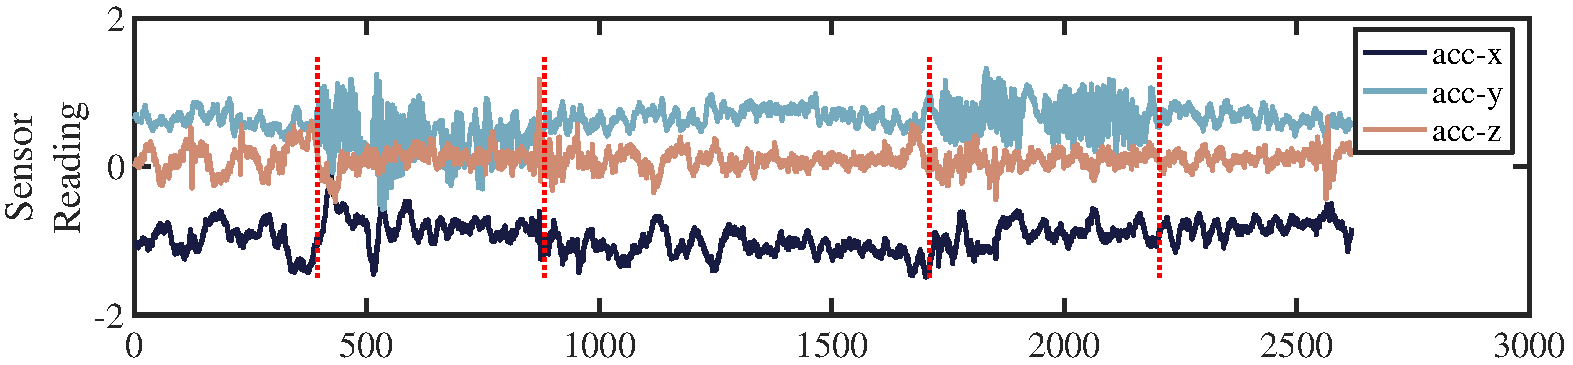
\includegraphics[width=\linewidth]{SPDC1}
		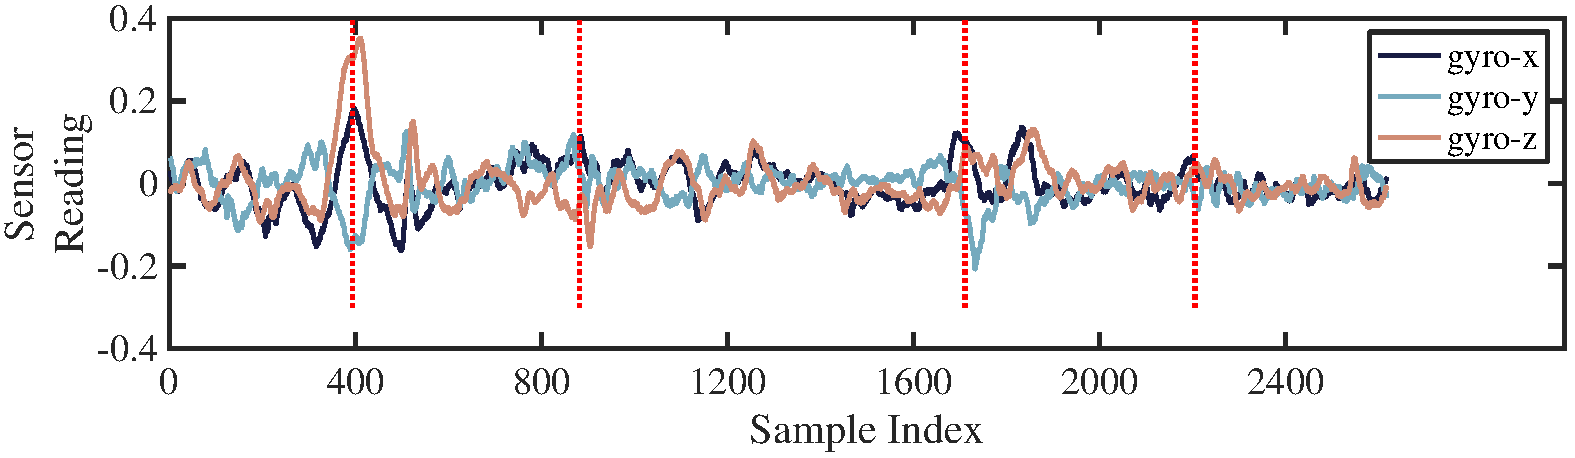
\includegraphics[width=\linewidth]{SPDC2}
		\vspace{-.2in}
		\subcaption{Raw Motion Data.}
		\vspace{.2in}
	\end{minipage}
	\begin{minipage}[t]{.45\linewidth}
		\centering
		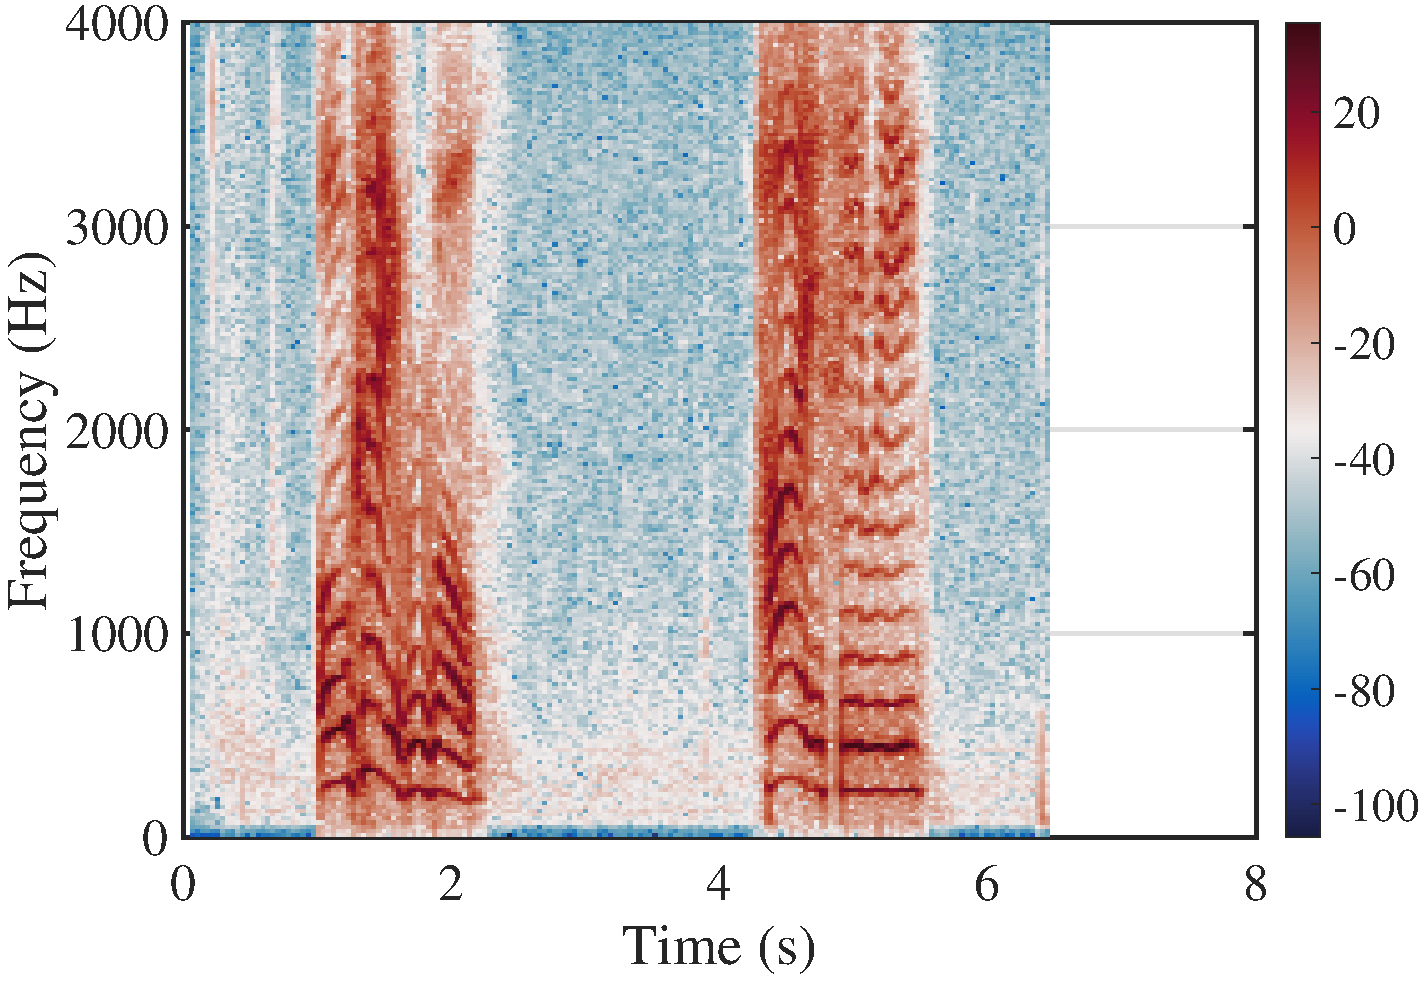
\includegraphics[width=\linewidth]{SPDC3}
		\vspace{-.2in}
		\subcaption{Spectrogram of Raw Audio Signals.}
	\end{minipage}
	\begin{minipage}[t]{.45\linewidth}
		\centering
		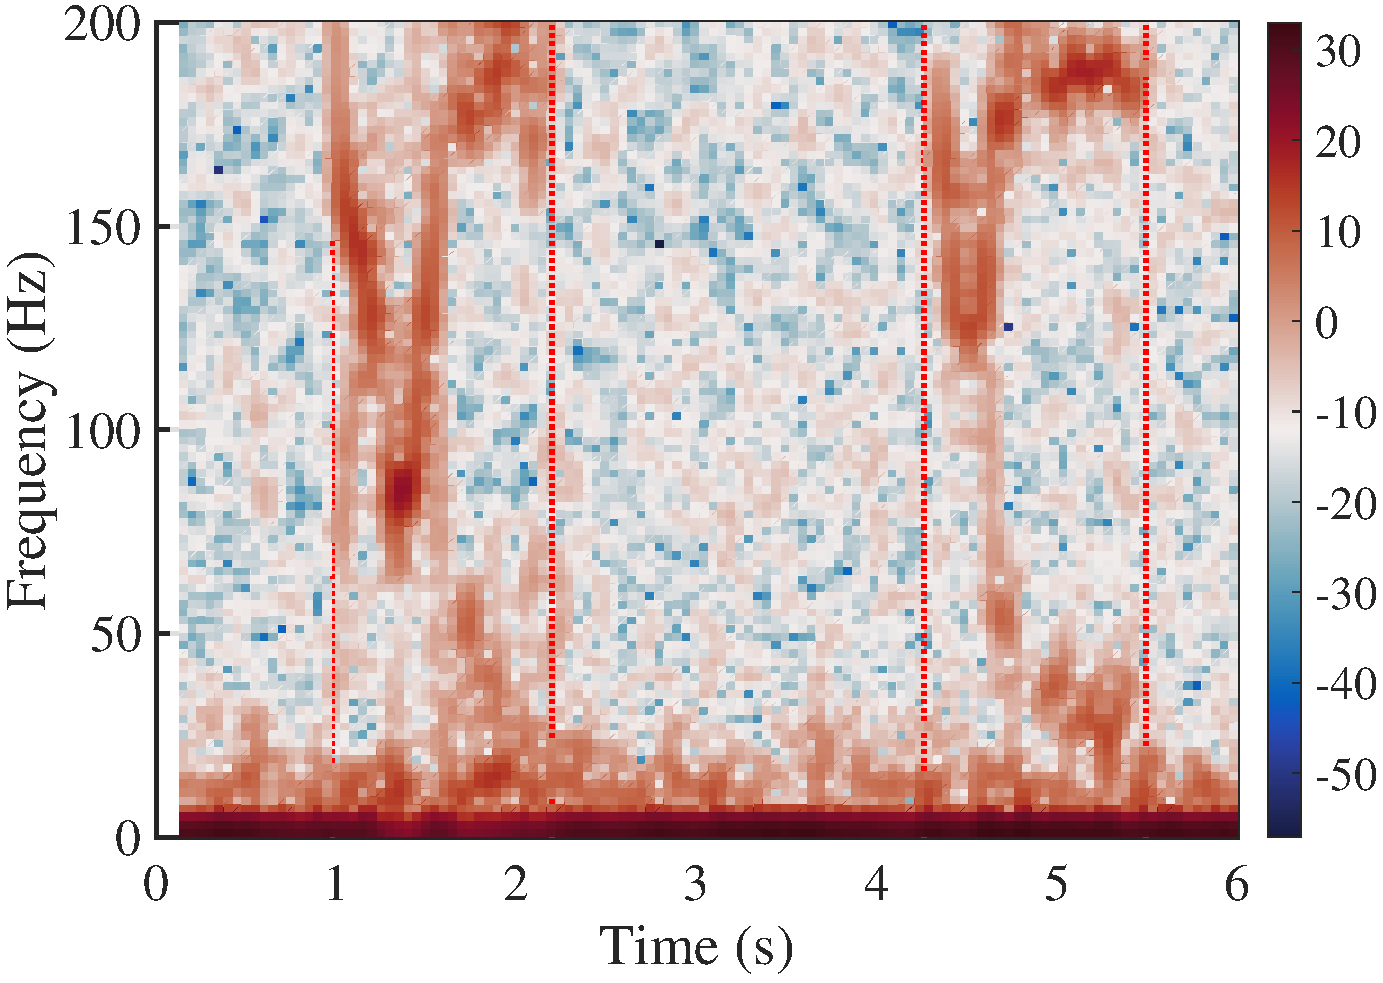
\includegraphics[width=\linewidth]{SPDC4}
		\vspace{-.2in}
		\subcaption{Spectrogram of Raw Motion Signals.}
	\end{minipage}
	\caption{One user speaks ``Ok Google'' and ``Hi Siri''.}
	\label{fig:SPDC}
\end{figure}
\newpage
\begin{figure}[H]
	\centering
	\begin{minipage}[t]{.8\linewidth}
		\centering
		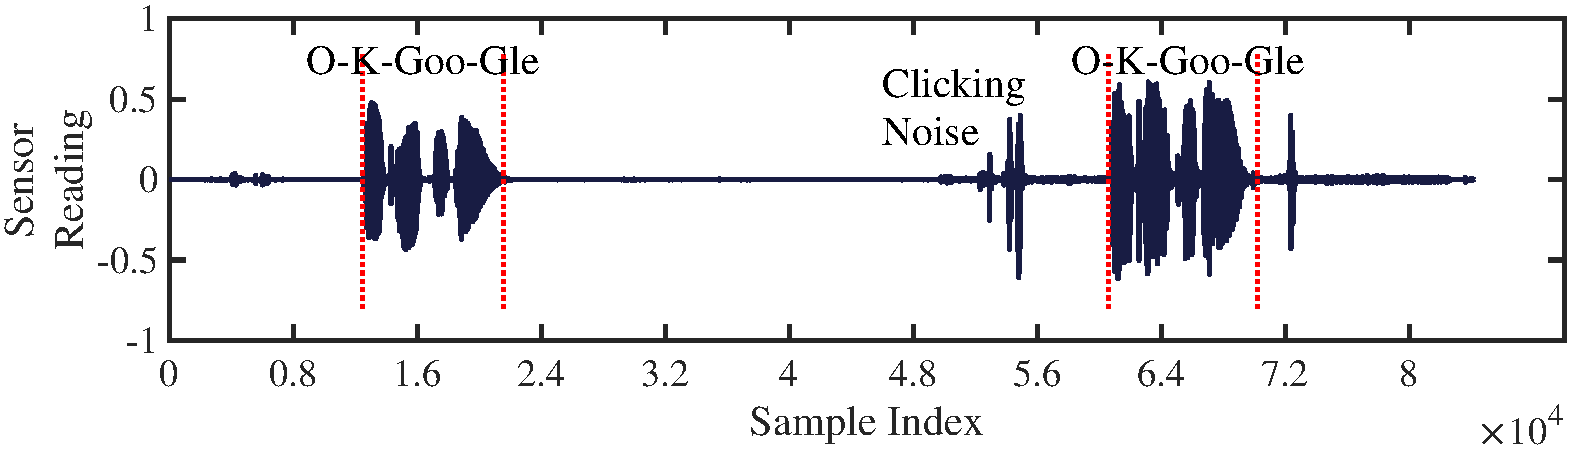
\includegraphics[width=\linewidth]{Device0}
		\vspace{-.2in}
		\subcaption{Raw Audio Data.}
		\vspace{.2in}
		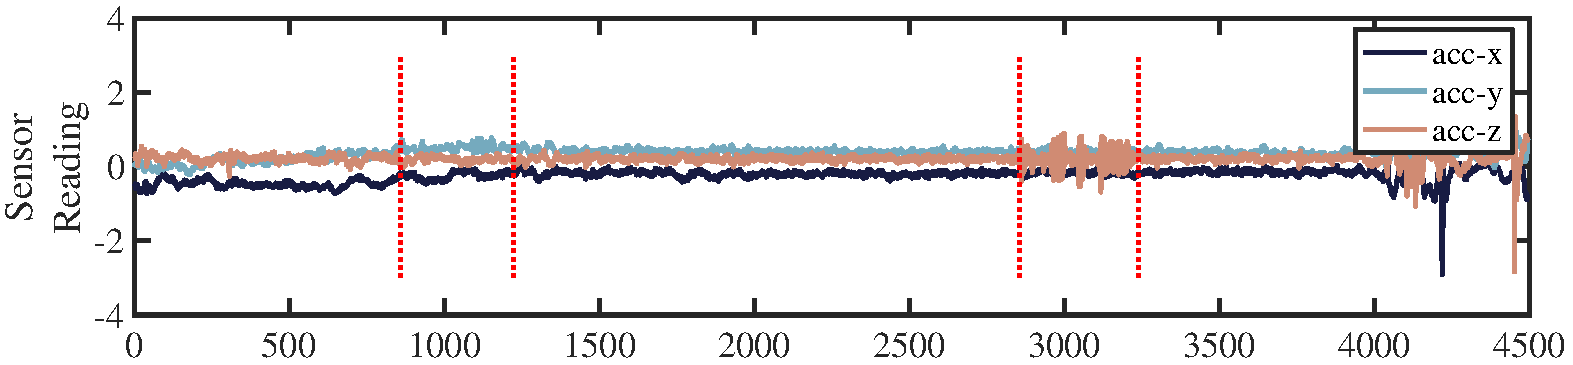
\includegraphics[width=\linewidth]{Device1}
		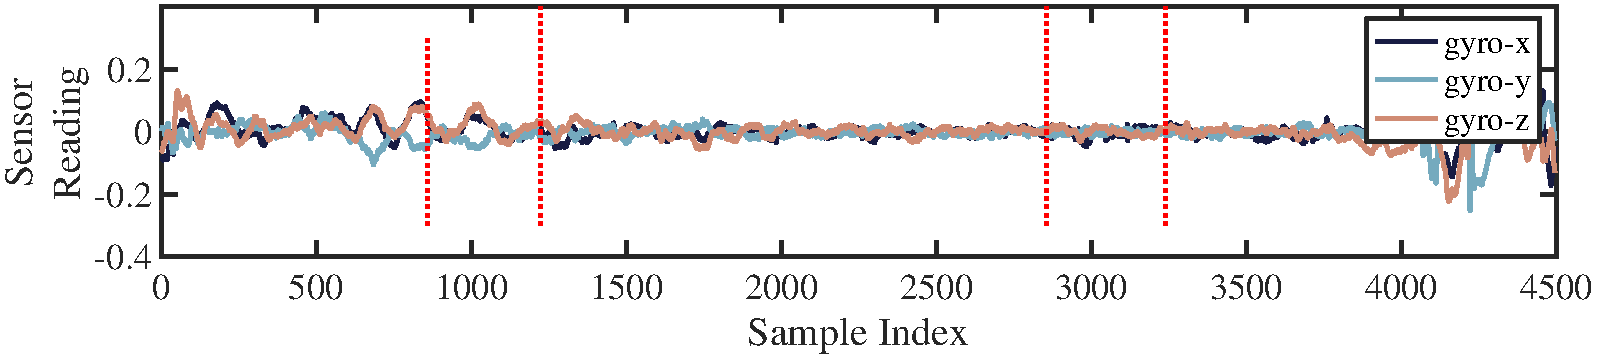
\includegraphics[width=\linewidth]{Device2}
		\vspace{-.2in}
		\subcaption{Raw Motion Data.}
		\vspace{.2in}
	\end{minipage}
	\begin{minipage}[t]{.45\linewidth}
		\centering
		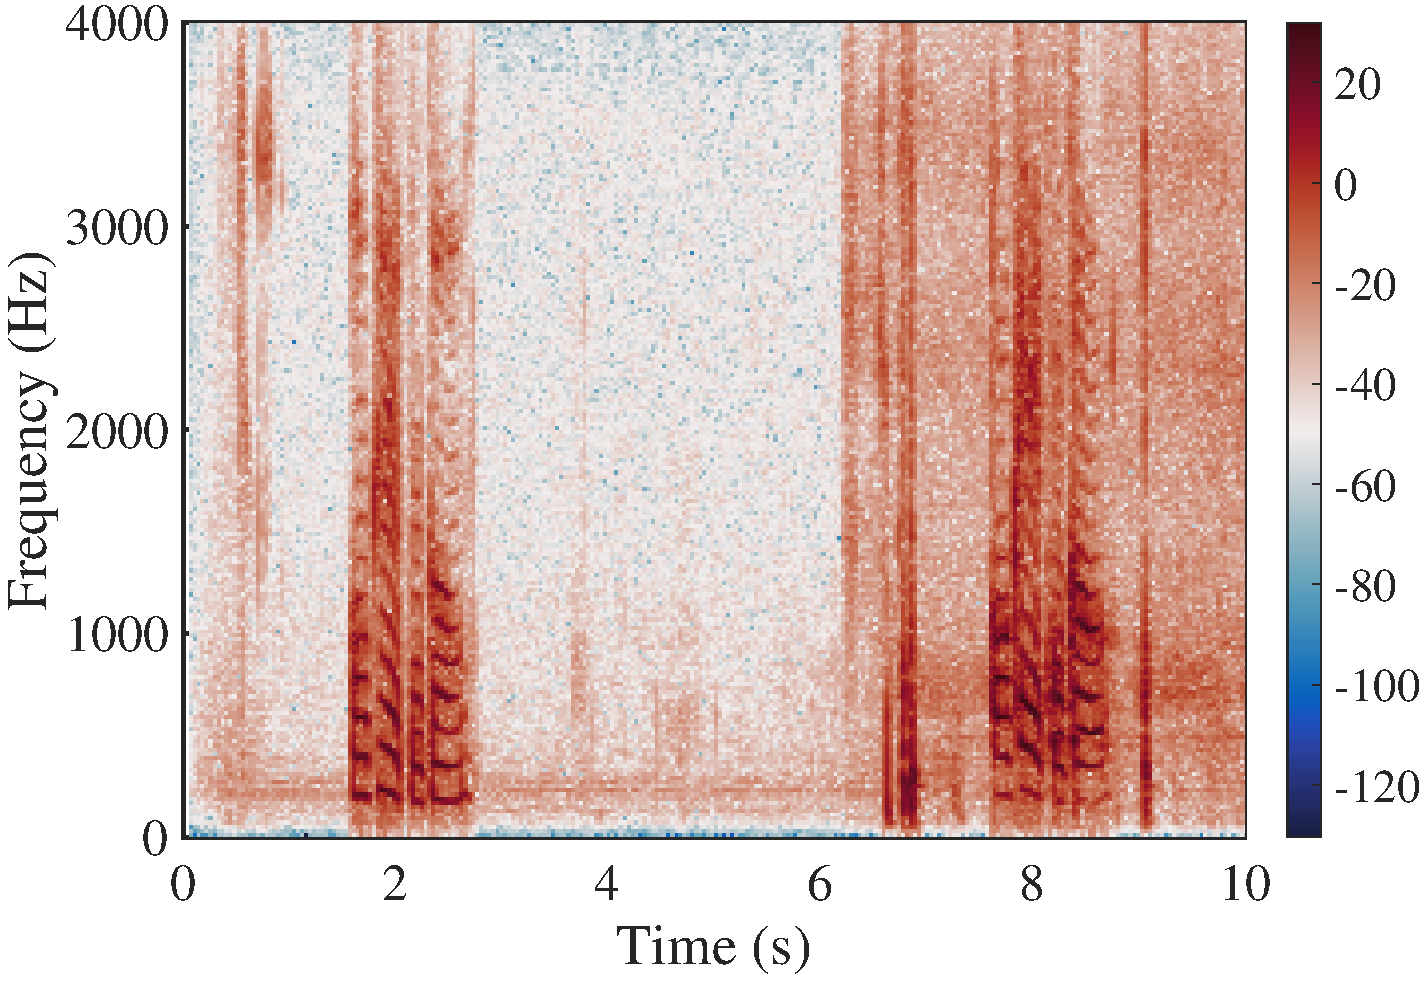
\includegraphics[width=\linewidth]{Device3}
		\vspace{-.2in}
		\subcaption{Spectrogram of Raw Audio Signals.}
	\end{minipage}
	\begin{minipage}[t]{.45\linewidth}
		\centering
		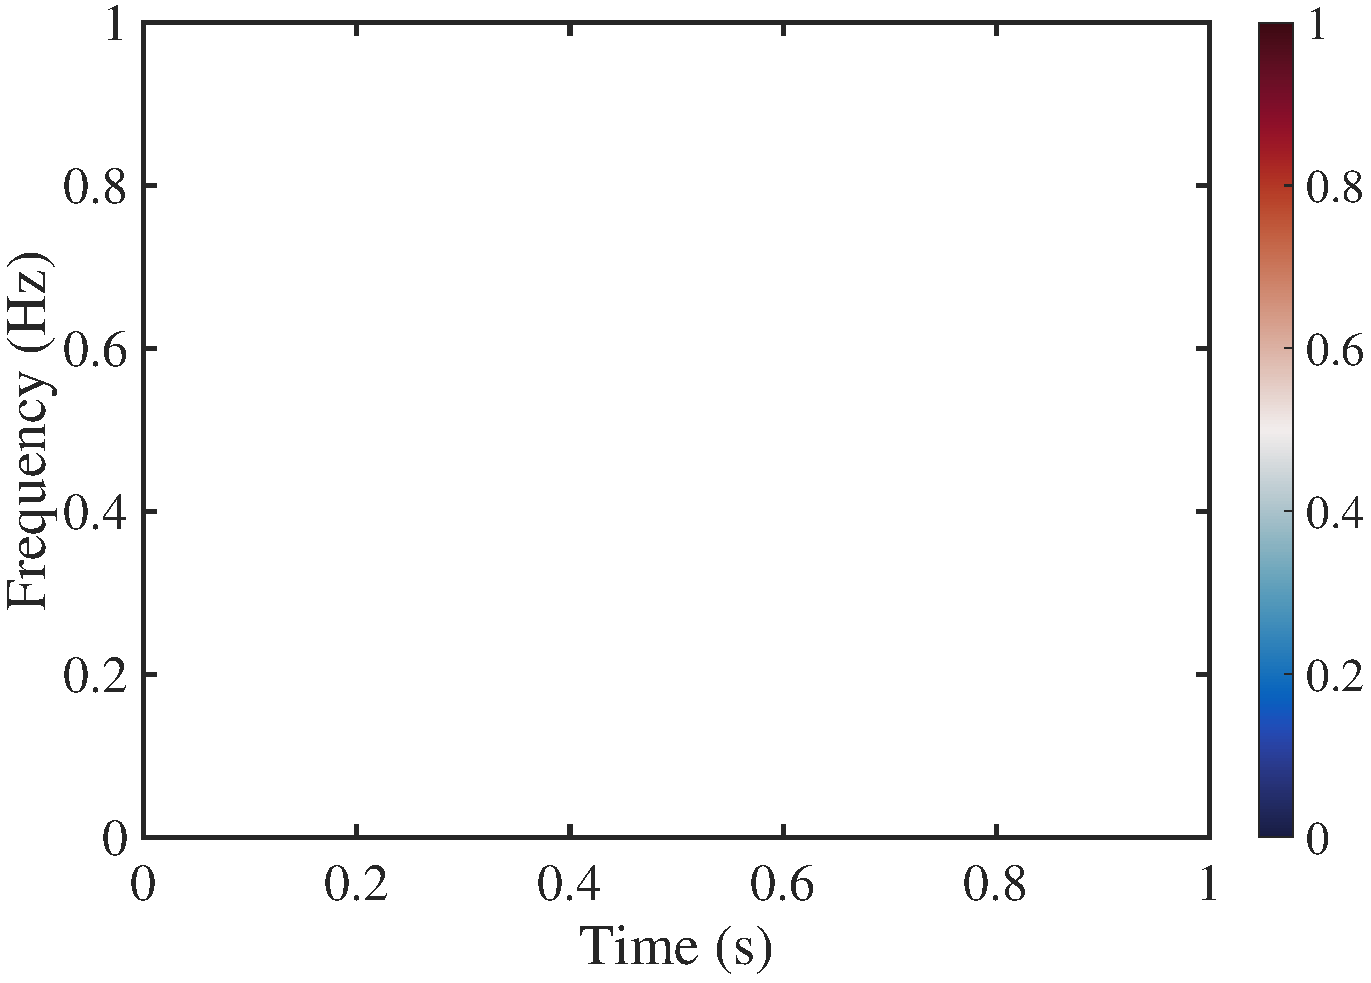
\includegraphics[width=\linewidth]{Device4}
		\vspace{-.2in}
		\subcaption{Spectrogram of Raw Motion Signals.}\label{fig:deviced}
	\end{minipage}
	\caption{Live user speaks ``Ok Google'' once, then replay the recording by electronic device.}
	\label{fig:device}
\end{figure}
\newpage


%TODO change same commands, do not fear DUPLICATION, ADDING HOW THE DATA IS COLLECTED
%todo NO ()

%TODO change plotted, are plotted, plot
%WHY CHOOSE AXIS-Z

%TODO

%
From these three figures, we can observe that the motion data are nosier and contain much fewer data and less representative than audio data, which indicates the challenge of designing {\shortname}. Fortunately, the results meet our expectation. Fig.~\ref{fig:SPSC} shows the consistence when the same user speaks the same command and Fig.~\ref{fig:DPSC} shows the difference when different users speak the same command. Such intra-class similarity and inter-class difference indicate the feasibility of using motion data for user authentication. Moreover, different users have similar raw audio spectrogram (Fig.~\ref{fig:DPSCc}) but different raw motion spectrogram (Fig.~\ref{fig:DPSCd}), which is an evidence of different acoustic attenuation effect of different people. Note that Fig.~\ref{fig:DPSCd} shows the spectrograms are similar when one user speaks different commands.  Such observations indicate that frequency-domain data are not of much use to match between motion data and the same commands. Therefore, we adopt long short-term memory (LSTM) network, a variant of recurrent neural network (RNN), to learn the patterns of motion data in time-domain. 


Fig.~\ref{fig:device} shows how {\shortname} can be spoof-proof. During the test, the user speaks ``Ok Google'' once, and two smartphones (one is Google Nexus 6P and the other is iPhone XS Max) record his voice. After the user finishes speaking, the iPhone XS Max replays the recordings to Nexus 6P. The replay volume is set to be the maximum possible and the two smartphones are physically contacted. The data in Fig.~\ref{fig:device} are the readings from Nexus 6P, which contains the live user's voice followed by the iPhone replayed voice. We observe that motion data for live person shows noticeable signals from 50 Hz to 200 Hz while motion data for electronic device shows only noises as in Fig.~\ref{fig:deviced}, which is an evidence of that the self demodulation effect of human body generates more low frequency signals (compared to original sound signals, the frequency of 50-200 Hz signals are low). Note that there exists a clicking noise at the time around 6.8 s, which is the time of clicking the button on iPhone to replay the voice. The iPhone is in close contact with the Nexus 6P, therefore the power of this clicking noise is very high.
%Note that in the ideal case, we expect when users speak the same command, no matter the same user or different users, the motion data should be similar. However, based on real data, as shown in Fig.~\ref{fig:DPSC} d), the raw spectrogram of different users are quite different. This is because different users have the different dominant speaking frequencies. What's worse, Fig.~\ref{fig:DPSC} d) shows the spectrograms are similar when one user speaks different commands.  Such observations indicate that frequency-domain data are not of much use to match between motion data and the same commands. Therefore, we adopt long short-term memory (LSTM) network, a variant of recurrent neural network (RNN), to learn the patterns of motion data in time-domain. 


%As elaborated in Section~\ref{sec:sys}, we also design syllable separation and majority voting components to further improve the performance of the LSTM network and increase the overall liveness detection accuracy.  In conclusion,  our \shortname~system has the following advantages:
%\begin{itemize}
%	\item \shortname~works with current-off-the-shelf commercial smartphones. It does not require any extra electronic device.
%	\item Except for pressing the smartphone on the user's throat, \shortname~does not ask users to do extra movements other than an ordinary speaking behavior. 
%	\item \shortname~can defend against at least 3*2= 6 different attacks. As elaborated in Section~\ref{sec:attack},  \shortname~protects the system against simple playback attack and sophisticated mimicry attack, where in each case, the speaker could play audio samples generated by replay attack, speech synthesis, or voice conversion. 
%	\item \shortname~does not require any user-specific training. Our matching algorithm is based on a user-independent model.
%	\item \shortname~currently works with text-dependent voice authentication systems. However, it is easy to expand the system to text-independent systems.
%\end{itemize}